% questions.tex —— 2011 年·辽宁卷·文科 · 题目内容片段（无答案）
% 由 tools/generate_projects.py 依来源总账自 2011/2011_数学真题_辽宁文_试题.md 生成，勿手改（改源 MD 后重跑）

\gkpart{一、选择题}

\begin{question}
\gkti{1}已知集合 $A=\{x\mid x>1\}$，$B=\{x\mid-1<x<2\}$，则 $A\cap B=$\mbox{（　　）}

（A）$\{x\mid-1<x<2\}$

（B）$\{x\mid x>-1\}$

（C）$\{x\mid-1<x<1\}$

（D）$\{x\mid1<x<2\}$

\end{question}
\begin{question}
\gkti{2}$\mathrm i$ 为虚数单位，$\dfrac1{\mathrm i}+\dfrac1{\mathrm i^3}+\dfrac1{\mathrm i^5}+\dfrac1{\mathrm i^7}=$\mbox{（　　）}

（A）$0$

（B）$2\mathrm i$

（C）$-2\mathrm i$

（D）$4\mathrm i$

\end{question}
\begin{question}
\gkti{3}已知向量 $\boldsymbol a=(2,1)$，$\boldsymbol b=(-1,k)$，$\boldsymbol a\cdot(2\boldsymbol a-\boldsymbol b)=0$，则 $k=$\mbox{（　　）}

（A）$-12$

（B）$-6$

（C）$6$

（D）$12$

\end{question}
\begin{question}
\gkti{4}已知命题 $p:\exists n\in\mathbf N$，$2^n>1000$，则 $\neg p$ 为\mbox{（　　）}

（A）$\forall n\in\mathbf N$，$2^n\leqslant1000$

（B）$\forall n\in\mathbf N$，$2^n>1000$

（C）$\exists n\in\mathbf N$，$2^n\leqslant1000$

（D）$\exists n\in\mathbf N$，$2^n<1000$

\end{question}
\begin{question}
\gkti{5}若等比数列 $\{a_n\}$ 满足 $a_na_{n+1}=16^n$，则公比为\mbox{（　　）}

（A）$2$

（B）$4$

（C）$8$

（D）$16$

\end{question}
\begin{question}
\gkti{6}若函数 $f(x)=\dfrac{x}{(2x+1)(x-a)}$ 为奇函数，则 $a=$\mbox{（　　）}

（A）$\frac12$

（B）$\frac23$

（C）$\frac34$

（D）$1$

\end{question}
\begin{question}
\gkti{7}已知 $F$ 是抛物线 $y^2=x$ 的焦点，$A$，$B$ 是该抛物线上的两点，$|AF|+|BF|=3$，则线段 $AB$ 的中点到 $y$ 轴的距离为\mbox{（　　）}

（A）$\frac34$

（B）$1$

（C）$\frac54$

（D）$\frac74$

\Needspace{0.4\textheight}
\end{question}
\begin{question}
\gkti{8}一个正三棱柱的侧棱长和底面边长相等，体积为 $2\sqrt3$，它的三视图中的俯视图如图所示，左视图是一个矩形，则这个矩形的面积是\mbox{（　　）}

（A）$4$

（B）$2\sqrt3$

（C）$2$

（D）$\sqrt3$
\nopagebreak[4]
\begin{center}% 2011 年辽宁卷文科第 8 题：正三棱柱俯视图（正三角形）。
% 来源 PDF：普通高考/2011/2011辽宁文.pdf，SHA-256 29407891a0a44aaa00db6398312f058fc98c005913323db3729a50333cec4564。
% 原页：第 1 页第 1 栏下部，书页码 683。
\begin{tikzpicture}[semithick, font=\small, scale=0.9]
  \coordinate (A) at (0,0);
  \coordinate (B) at (2.4,0);
  \coordinate (C) at (1.2,2.078);
  \draw[thick] (A)--(B)--(C)--cycle;
  \node[below] at (1.2,-0.32) {俯视图};
\end{tikzpicture}
\end{center}
\nopagebreak[4]
\Needspace{0.4\textheight}
\end{question}
\begin{question}
\gkti{9}执行下面的程序框图，如果输入的 $n$ 是 $4$，则输出的 $p$ 是\mbox{（　　）}

（A）$8$

（B）$5$

（C）$3$

（D）$2$
\nopagebreak[4]
\begin{center}% 2011 年辽宁卷文科第 9 题：程序框图。
% 来源 PDF：普通高考/2011/2011辽宁文.pdf，SHA-256 29407891a0a44aaa00db6398312f058fc98c005913323db3729a50333cec4564。
% 原页：第 1 页第 2 栏上部，书页码 683。
\begin{tikzpicture}[>=stealth, semithick, font=\small, node distance=6mm]
  \node[draw, rounded corners=0.12cm, minimum width=1.5cm, minimum height=0.5cm] (start) {开始};
  \node[draw, trapezium, trapezium left angle=72, trapezium right angle=108,
        minimum width=1.8cm, minimum height=0.55cm, below=of start] (in) {输入 $n$};
  \node[draw, minimum width=3.6cm, minimum height=0.55cm, below=of in] (init)
        {$s=0$，$t=1$，$k=1$，$p=1$};
  \node[draw, diamond, aspect=2.1, minimum width=2.0cm, minimum height=0.95cm, below=of init] (test) {$k<n$};
  \node[draw, minimum width=1.8cm, minimum height=0.5cm, below=of test] (p) {$p=s+t$};
  \node[draw, minimum width=2.2cm, minimum height=0.5cm, below=of p] (st) {$s=t$，$t=p$};
  \node[draw, minimum width=1.8cm, minimum height=0.5cm, below=of st] (k) {$k=k+1$};
  \node[draw, trapezium, trapezium left angle=72, trapezium right angle=108,
        minimum width=1.8cm, minimum height=0.55cm, below=of k] (out) {输出 $p$};
  \node[draw, rounded corners=0.12cm, minimum width=1.5cm, minimum height=0.5cm, below=of out] (stop) {结束};
  \draw[->] (start)--(in);
  \draw[->] (in)--(init);
  \draw[->] (init)--(test);
  \draw[->] (test)--node[right] {是} (p);
  \draw[->] (p)--(st);
  \draw[->] (st)--(k);
  \draw[->] (k.west) -- ++(-1.4,0) |- (test.west);
  \draw[->] (test.east) -- ++(1.6,0) node[pos=0.4, above] {否} |- (out.east);
  \draw[->] (out)--(stop);
\end{tikzpicture}
\end{center}
\nopagebreak[4]
\end{question}
\begin{question}
\gkti{10}已知球的直径 $SC=4$，$A$，$B$ 是该球球面上的两点，$AB=2$，$\angle ASC=\angle BSC=45^\circ$，则棱锥 $S-ABC$ 的体积为\mbox{（　　）}

（A）$\frac{\sqrt3}3$

（B）$\frac{2\sqrt3}3$

（C）$\frac{4\sqrt3}3$

（D）$\frac{5\sqrt3}3$

\end{question}
\begin{question}
\gkti{11}函数 $f(x)$ 的定义域为 $\mathbf R$，$f(-1)=2$，对任意 $x\in\mathbf R$，$f'(x)>2$，则 $f(x)>2x+4$ 的解集为\mbox{（　　）}

（A）$(-1,1)$

（B）$(-1,+\infty)$

（C）$(-\infty,-1)$

（D）$(-\infty,+\infty)$

\Needspace{0.4\textheight}
\end{question}
\begin{question}
\gkti{12}已知函数 $f(x)=A\tan(\omega x+\varphi)$（$\omega>0$，$|\varphi|<\dfrac\pi2$），$y=f(x)$ 的部分图象如图，则 $f\left(\dfrac\pi{24}\right)=$\mbox{（　　）}

（A）$2+\sqrt3$

（B）$\sqrt3$

（C）$\frac{\sqrt3}3$

（D）$2-\sqrt3$
\nopagebreak[4]
\begin{center}% 2011 年辽宁卷文科第 12 题：y=A tan(ωx+φ) 的部分图象。
% 来源 PDF：普通高考/2011/2011辽宁文.pdf，SHA-256 29407891a0a44aaa00db6398312f058fc98c005913323db3729a50333cec4564。
% 原页：第 1 页第 2 栏中部，书页码 683。图象对应 f(x)=tan(2x+π/4)。
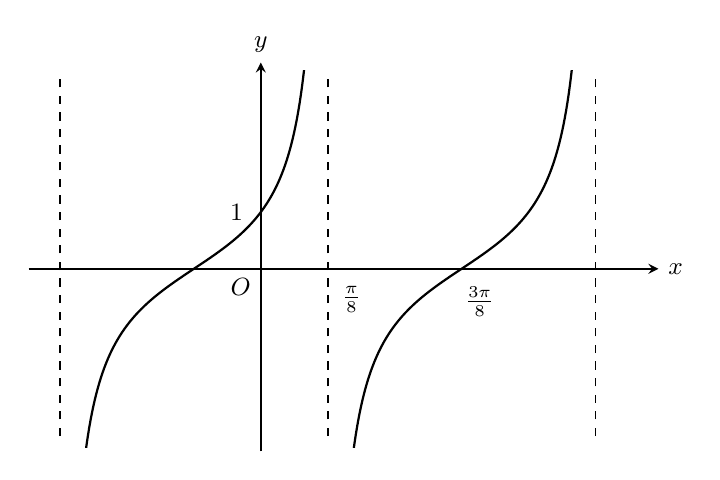
\begin{tikzpicture}[>=stealth, semithick, font=\small]
  \begin{scope}[xscale=0.85, yscale=0.72]
    \clip (-3.45,-3.15) rectangle (5.7,3.5);
    \draw[thick] plot[domain=-2.98:0.98, samples=200] (\x,{tan((\x+1)*45)});
    \draw[thick] plot[domain=1.02:4.98, samples=200] (\x,{tan((\x+1)*45)});
    \foreach \a in {-3,1,5} {
      \draw[dashed] (\a,-2.95)--(\a,3.4);
    }
  \end{scope}
  \draw[->] (-2.95,0)--(5.05,0) node[right] {$x$};
  \draw[->] (0,-2.32)--(0,2.62) node[above] {$y$};
  \node[below left] at (0,0) {$O$};
  \node[left] at (-0.1,0.72) {$1$};
  \node[below] at (1.15,-0.10) {$\frac{\pi}{8}$};
  \node[below] at (2.78,-0.10) {$\frac{3\pi}{8}$};
\end{tikzpicture}
\end{center}
\nopagebreak[4]
\end{question}
\gkpart{二、填空题}

\begin{question}
\gkti{13}已知圆 $C$ 经过 $A(5,1)$，$B(1,3)$ 两点，圆心在 $x$ 轴上，则 $C$ 的方程为 $\underline{\qquad}$。

\end{question}
\begin{question}
\gkti{14}调查了某地若干户家庭的年收入 $x$（单位：万元）和年饮食支出 $y$（单位：万元），调查显示年收入 $x$ 与年饮食支出 $y$ 具有线性相关关系，并由调查数据得到 $y$ 对 $x$ 的回归直线方程：$\hat y=0.254x+0.321$。由回归直线方程可知，家庭年收入每增加 $1$ 万元，年饮食支出平均增加 $\underline{\qquad}$ 万元。

\end{question}
\begin{question}
\gkti{15}$S_n$ 为等差数列 $\{a_n\}$ 的前 $n$ 项和，$S_2=S_6$，$a_4=1$，则 $a_5=\underline{\qquad}$。

\end{question}
\begin{question}
\gkti{16}已知函数 $f(x)=\mathrm e^x-2x+a$ 有零点，则 $a$ 的取值范围是 $\underline{\qquad}$。

\end{question}
\gkpart{三、解答题}

\begin{question}
\gkti{17}$\triangle ABC$ 的三个内角 $A$，$B$，$C$ 所对的边分别为 $a$，$b$，$c$，$a\sin A\sin B+b\cos^2A=\sqrt2a$。

（1） 求 $\dfrac ba$；

（2） 若 $c^2=b^2+\sqrt3a^2$，求 $B$。

\Needspace{0.4\textheight}
\end{question}
\begin{question}
\gkti{18}如图，四边形 $ABCD$ 为正方形，$QA\perp$ 平面 $ABCD$，$PD\parallel QA$，$QA=AB=\dfrac12PD$。

（1） 证明：$PQ\perp$ 平面 $DCQ$；

（2） 求棱锥 $Q-ABCD$ 的体积与棱锥 $P-DCQ$ 的体积比值。
\nopagebreak[4]
\begin{center}% 2011 年辽宁卷文科第 18 题：正方形 ABCD，QA⊥平面 ABCD，PD∥QA。
% 来源 PDF：普通高考/2011/2011辽宁文.pdf，SHA-256 29407891a0a44aaa00db6398312f058fc98c005913323db3729a50333cec4564。
% 原页：第 1 页第 3 栏下部，书页码 683。示意。
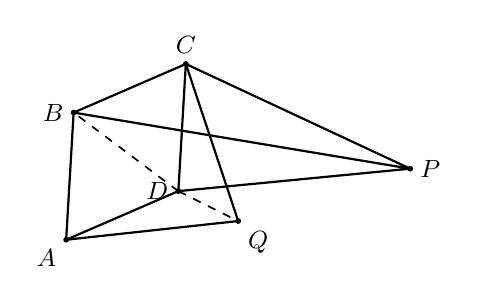
\begin{tikzpicture}[>=stealth, semithick, font=\small, scale=0.95]
  \coordinate (A) at (0,0);
  \coordinate (B) at (0.1,1.7);
  \coordinate (C) at (1.6,2.35);
  \coordinate (D) at (1.5,0.65);
  \coordinate (P) at (4.6,0.95);
  \coordinate (Q) at (2.3,0.25);
  \draw[thick] (A)--(B)--(C)--(D)--cycle;
  \draw[thick] (P)--(D) (P)--(C) (P)--(B);
  \draw[thick] (Q)--(A) (Q)--(C);
  \draw[dashed] (D)--(B) (D)--(Q);
  \fill (A) circle (1.1pt) node[below left] {$A$};
  \fill (B) circle (1.1pt) node[left] {$B$};
  \fill (C) circle (1.1pt) node[above] {$C$};
  \fill (D) circle (1.1pt) node[left] {$D$};
  \fill (P) circle (1.1pt) node[right] {$P$};
  \fill (Q) circle (1.1pt) node[below right] {$Q$};
\end{tikzpicture}
\end{center}
\nopagebreak[4]
\end{question}
\begin{question}
\gkti{19}某农场计划种植某种新作物，为此对这种作物的两个品种（分别称为品种甲和品种乙）进行田间试验，选取两大块地，每大块地分成 $n$ 小块地，在总共 $2n$ 小块地中，随机选 $n$ 小块地种植品种甲，另外 $n$ 小块地种植品种乙。

（1） 假设 $n=2$，求第一大块地都种植品种甲的概率；

（2） 试验时每大块地分成 $8$ 小块，即 $n=8$，试验结束后得到品种甲和品种乙在各小块地上的每公顷产量（单位：$\mathrm{kg/hm^2}$）如下表：

\begin{center}
\begingroup\setlength{\tabcolsep}{4pt}
\begin{tabular}{lllllllll}
\toprule
品种甲 & 403 & 397 & 390 & 404 & 388 & 400 & 412 & 406 \\
\midrule
品种乙 & 419 & 403 & 412 & 418 & 408 & 423 & 400 & 413 \\
\bottomrule
\end{tabular}
\endgroup
\end{center}

分别求品种甲和品种乙每公顷产量的样本平均数和样本方差；根据试验结果，你应该种植哪一品种？

\Needspace{5\baselineskip}
附：样本数据 $x_1,x_2,\cdots,x_n$ 的样本方差

\nopagebreak[4]
\[\begin{aligned}
s^2={}&\frac1n\bigl[(x_1-\bar x)^2+(x_2-\bar x)^2\\
&+\cdots+(x_n-\bar x)^2\bigr],
\end{aligned}\]

其中 $\bar x$ 为样本平均数。

\end{question}
\begin{question}
\gkti{20}设函数 $f(x)=x+ax^2+b\ln x$，曲线 $y=f(x)$ 过 $P(1,0)$，且在 $P$ 点处的切线斜率为 $2$。

（1） 求 $a$，$b$ 的值；

（2） 证明：$f(x)\leqslant2x-2$。

\Needspace{0.4\textheight}
\end{question}
\begin{question}
\gkti{21}如图，已知椭圆 $C_1$ 的中心在原点 $O$，长轴左、右端点 $M$，$N$ 在 $x$ 轴上，椭圆 $C_2$ 的短轴为 $MN$，且 $C_1$，$C_2$ 的离心率都为 $e$。直线 $l\perp MN$，$l$ 与 $C_1$ 交于两点，与 $C_2$ 交于两点，这四点按纵坐标从大到小依次为 $A$，$B$，$C$，$D$。

（1） 设 $e=\dfrac12$，求 $|BC|$ 与 $|AD|$ 的比值；

（2） 当 $e$ 变化时，是否存在直线 $l$，使得 $BO\parallel AN$，并说明理由。
\nopagebreak[4]
\begin{center}% 2011 年辽宁卷文科第 21 题：椭圆 C1、C2 与直线 l。
% 来源 PDF：普通高考/2011/2011辽宁文.pdf，SHA-256 29407891a0a44aaa00db6398312f058fc98c005913323db3729a50333cec4564。
% 原页：第 2 页第 2 栏中部，书页码 684。示意。
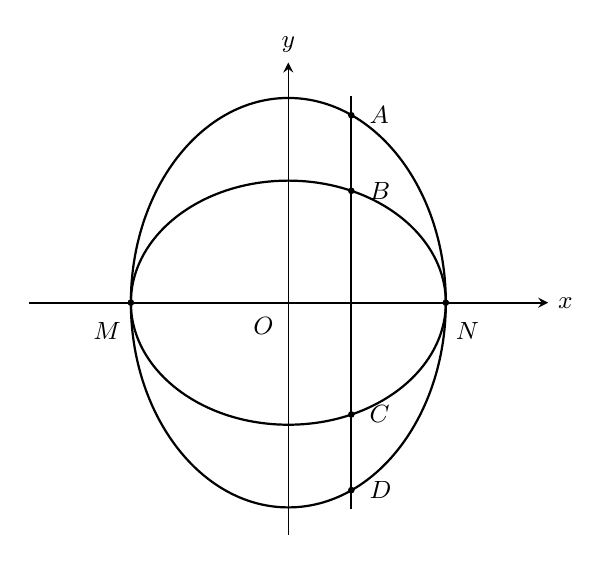
\begin{tikzpicture}[>=stealth, semithick, font=\small, scale=1.0]
  \draw[->] (-3.3,0)--(3.3,0) node[right] {$x$};
  \draw[->] (0,-2.95)--(0,3.05) node[above] {$y$};
  \draw[thick] (0,0) ellipse (2 and 1.55);
  \draw[thick] (0,0) ellipse (2 and 2.6);
  \draw[thick] (0.8,-2.62)--(0.8,2.62);
  \fill (0.8,2.38) circle (1.2pt) node[right=3pt] {$A$};
  \fill (0.8,1.42) circle (1.2pt) node[right=3pt] {$B$};
  \fill (0.8,-1.42) circle (1.2pt) node[right=3pt] {$C$};
  \fill (0.8,-2.38) circle (1.2pt) node[right=3pt] {$D$};
  \fill (-2,0) circle (1.2pt);
  \fill (2,0) circle (1.2pt);
  \node[below left] at (-2,-0.12) {$M$};
  \node[below right] at (2,-0.12) {$N$};
  \node[below left] at (-0.06,-0.06) {$O$};
\end{tikzpicture}
\end{center}
\nopagebreak[4]
\Needspace{0.4\textheight}
\end{question}
\begin{question}
\gkti{22}三选一。

【A】如图，$A$，$B$，$C$，$D$ 四点在同一圆上，$AD$ 的延长线与 $BC$ 的延长线交于 $E$ 点，且 $EC=ED$。

（1） 证明：$CD\parallel AB$；

（2） 延长 $CD$ 到 $F$，延长 $DC$ 到 $G$，使得 $EF=EG$，证明：$A$，$B$，$G$，$F$ 四点共圆。
\nopagebreak[4]
\begin{center}% 2011 年辽宁卷文科第 22A 题：四点共圆与两割线。
% 来源 PDF：普通高考/2011/2011辽宁文.pdf，SHA-256 29407891a0a44aaa00db6398312f058fc98c005913323db3729a50333cec4564。
% 原页：第 2 页第 2 栏下部，书页码 684。示意。
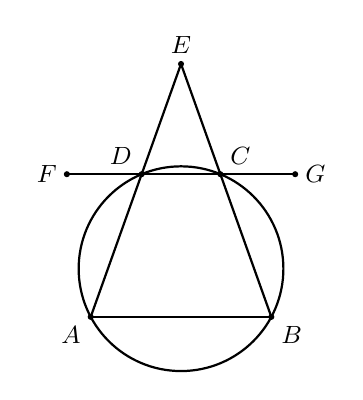
\begin{tikzpicture}[>=stealth, semithick, font=\small, scale=1.0]
  \draw[thick] (0,0) circle (1.3);
  \coordinate (E) at (0,2.6);
  \coordinate (D) at (-0.5,1.2);
  \coordinate (C) at (0.5,1.2);
  \coordinate (A) at (-1.147,-0.612);
  \coordinate (B) at (1.147,-0.612);
  \coordinate (F) at (-1.45,1.2);
  \coordinate (G) at (1.45,1.2);
  \draw[thick] (E)--(A);
  \draw[thick] (E)--(B);
  \draw[thick] (F)--(G);
  \draw (A)--(B);
  \fill (E) circle (1.1pt) node[above] {$E$};
  \fill (F) circle (1.1pt) node[left] {$F$};
  \fill (G) circle (1.1pt) node[right] {$G$};
  \fill (D) circle (1.1pt) node[above left] {$D$};
  \fill (C) circle (1.1pt) node[above right] {$C$};
  \fill (A) circle (1.1pt) node[below left] {$A$};
  \fill (B) circle (1.1pt) node[below right] {$B$};
\end{tikzpicture}
\end{center}
\nopagebreak[4]
【B】在平面直角坐标系 $xOy$ 中，曲线 $C_1$ 的参数方程为 $\begin{cases}x=\cos\varphi,\\y=\sin\varphi,\end{cases}$（$\varphi$ 为参数），曲线 $C_2$ 的参数方程为 $\begin{cases}x=a\cos\varphi,\\y=b\sin\varphi,\end{cases}$（$a>b>0$，$\varphi$ 为参数）。在以 $O$ 为极点，$x$ 轴的正半轴为极轴的极坐标系中，射线 $l:\theta=\alpha$ 与 $C_1$，$C_2$ 各有一个交点，当 $\alpha=0$ 时，这两个交点间的距离为 $2$，当 $\alpha=\dfrac\pi2$ 时，这两个交点重合。

（1） 分别说明 $C_1$，$C_2$ 是什么曲线，并求出 $a$ 与 $b$ 的值；

（2） 设当 $\alpha=\dfrac\pi4$ 时，$l$ 与 $C_1$，$C_2$ 的交点分别为 $A_1$，$B_1$，当 $\alpha=-\dfrac\pi4$ 时，$l$ 与 $C_1$，$C_2$ 的交点分别为 $A_2$，$B_2$，求四边形 $A_1A_2B_2B_1$ 的面积。

【C】已知函数 $f(x)=|x-2|-|x-5|$。

（1） 证明：$-3\leqslant f(x)\leqslant3$；

（2） 求不等式 $f(x)\geqslant x^2-8x+15$ 的解集。

\end{question}